
\section{Appendix: $G$-statistic}\label{sec:Gapp}
As was previously mentioned, the $F_1$-statistic outperforms all variants of the $G$-statistic, but the formal sensitivity analysis and optimizations are provided for the few use cases where the $G$-statistic is more powerful. 
%\subsection{Optimal exponent for $G$}
%Much like the $F_2$ statistic, we wondered what the optimal exponent on the statistic would be.
  As with the previous statistics, we need to bound the sensitivity of \varq to use the Laplace mechanism (Definition~\ref{thm:lapmechanism}).

\begin{theorem}[\varq-Sensitivity] \label{thm:varqSens} 
The sensitivity of \varq is bounded above by
$$ \frac{N-1}{N^q} + 1 $$
when $q<1$, and is bounded above by
$$ (N-1)(1-(1-1/N)^q) + 1 $$
when $q>1$. Note that these both give a bound of $2-1/N$ when $q=1$.
\end{theorem}

\begin{proof}
Consider databases \x and \xprime which differ in entry $r$. Recall that the sensitivity of the grand mean is $1/N$. Let $t_i = \left\vert  y_i - \grand \right\vert ^q$. When $q<1, t_i$ is a concave function with positive range, so the worst case sensitivity is between $ y_i - \grand = 0$ and $ y_i - \grand = 1/N$. That is, 
\begin{align*}
\Delta t_i &= \left\vert t_{i}(0) - t_i\left(\frac{1}{N}\right) \right\vert \\
	&= \left( \frac{1}{N} \right)^q.
\end{align*}
%
Every single term can be affected by at most $\left( \frac{1}{N} \right)^q$, except the term $r$, which can change by $1$. So, 
\begin{align*}
\Delta \varq &\le \left\vert (N-1)(\frac{1}{N})^q + 1 \right\vert \\
	&= \frac{N-1}{N^q} + 1.
\end{align*}
%
When $q>1, t_i$ is convex. The worst case sensitivity is between  $y_i - \grand = 1$ and $y_i - \grand = 1-1/N$ Then,
\begin{align*}
\Delta \varq \le \left\vert (N-1)(1-(1-\frac{1}{N})^q) + 1 \right\vert.
\end{align*}
\end{proof}


%In order to run these statistics on simulated data, we used the Laplacian Mechanism as before (Theorem~\ref{thm:lapmechanism}). We also used the same method for computing $p$-values as the method described for the $F_1$-statistic (Algorithm~\ref{alg:pval}).

We ran the $G$-statistics on simulated data, using the same method for computing $p$-values as the method described for the $F_1$-statistic (Algorithm~\ref{alg:pval}).    We found that $q=1$ is the ideal exponent for the $G$-statistic for simulations that used the true database standard deviation (Figure~\ref{fig:Gpexponents}). For the remaining sections, we will be using the $\var_1 \cdot \sqrt{\pi/2}$ as the standard deviation estimate for the $G_1$-statistic because $\var_1$ and \se are drawn from the half-normal distribution. 
\begin{figure}
\centering
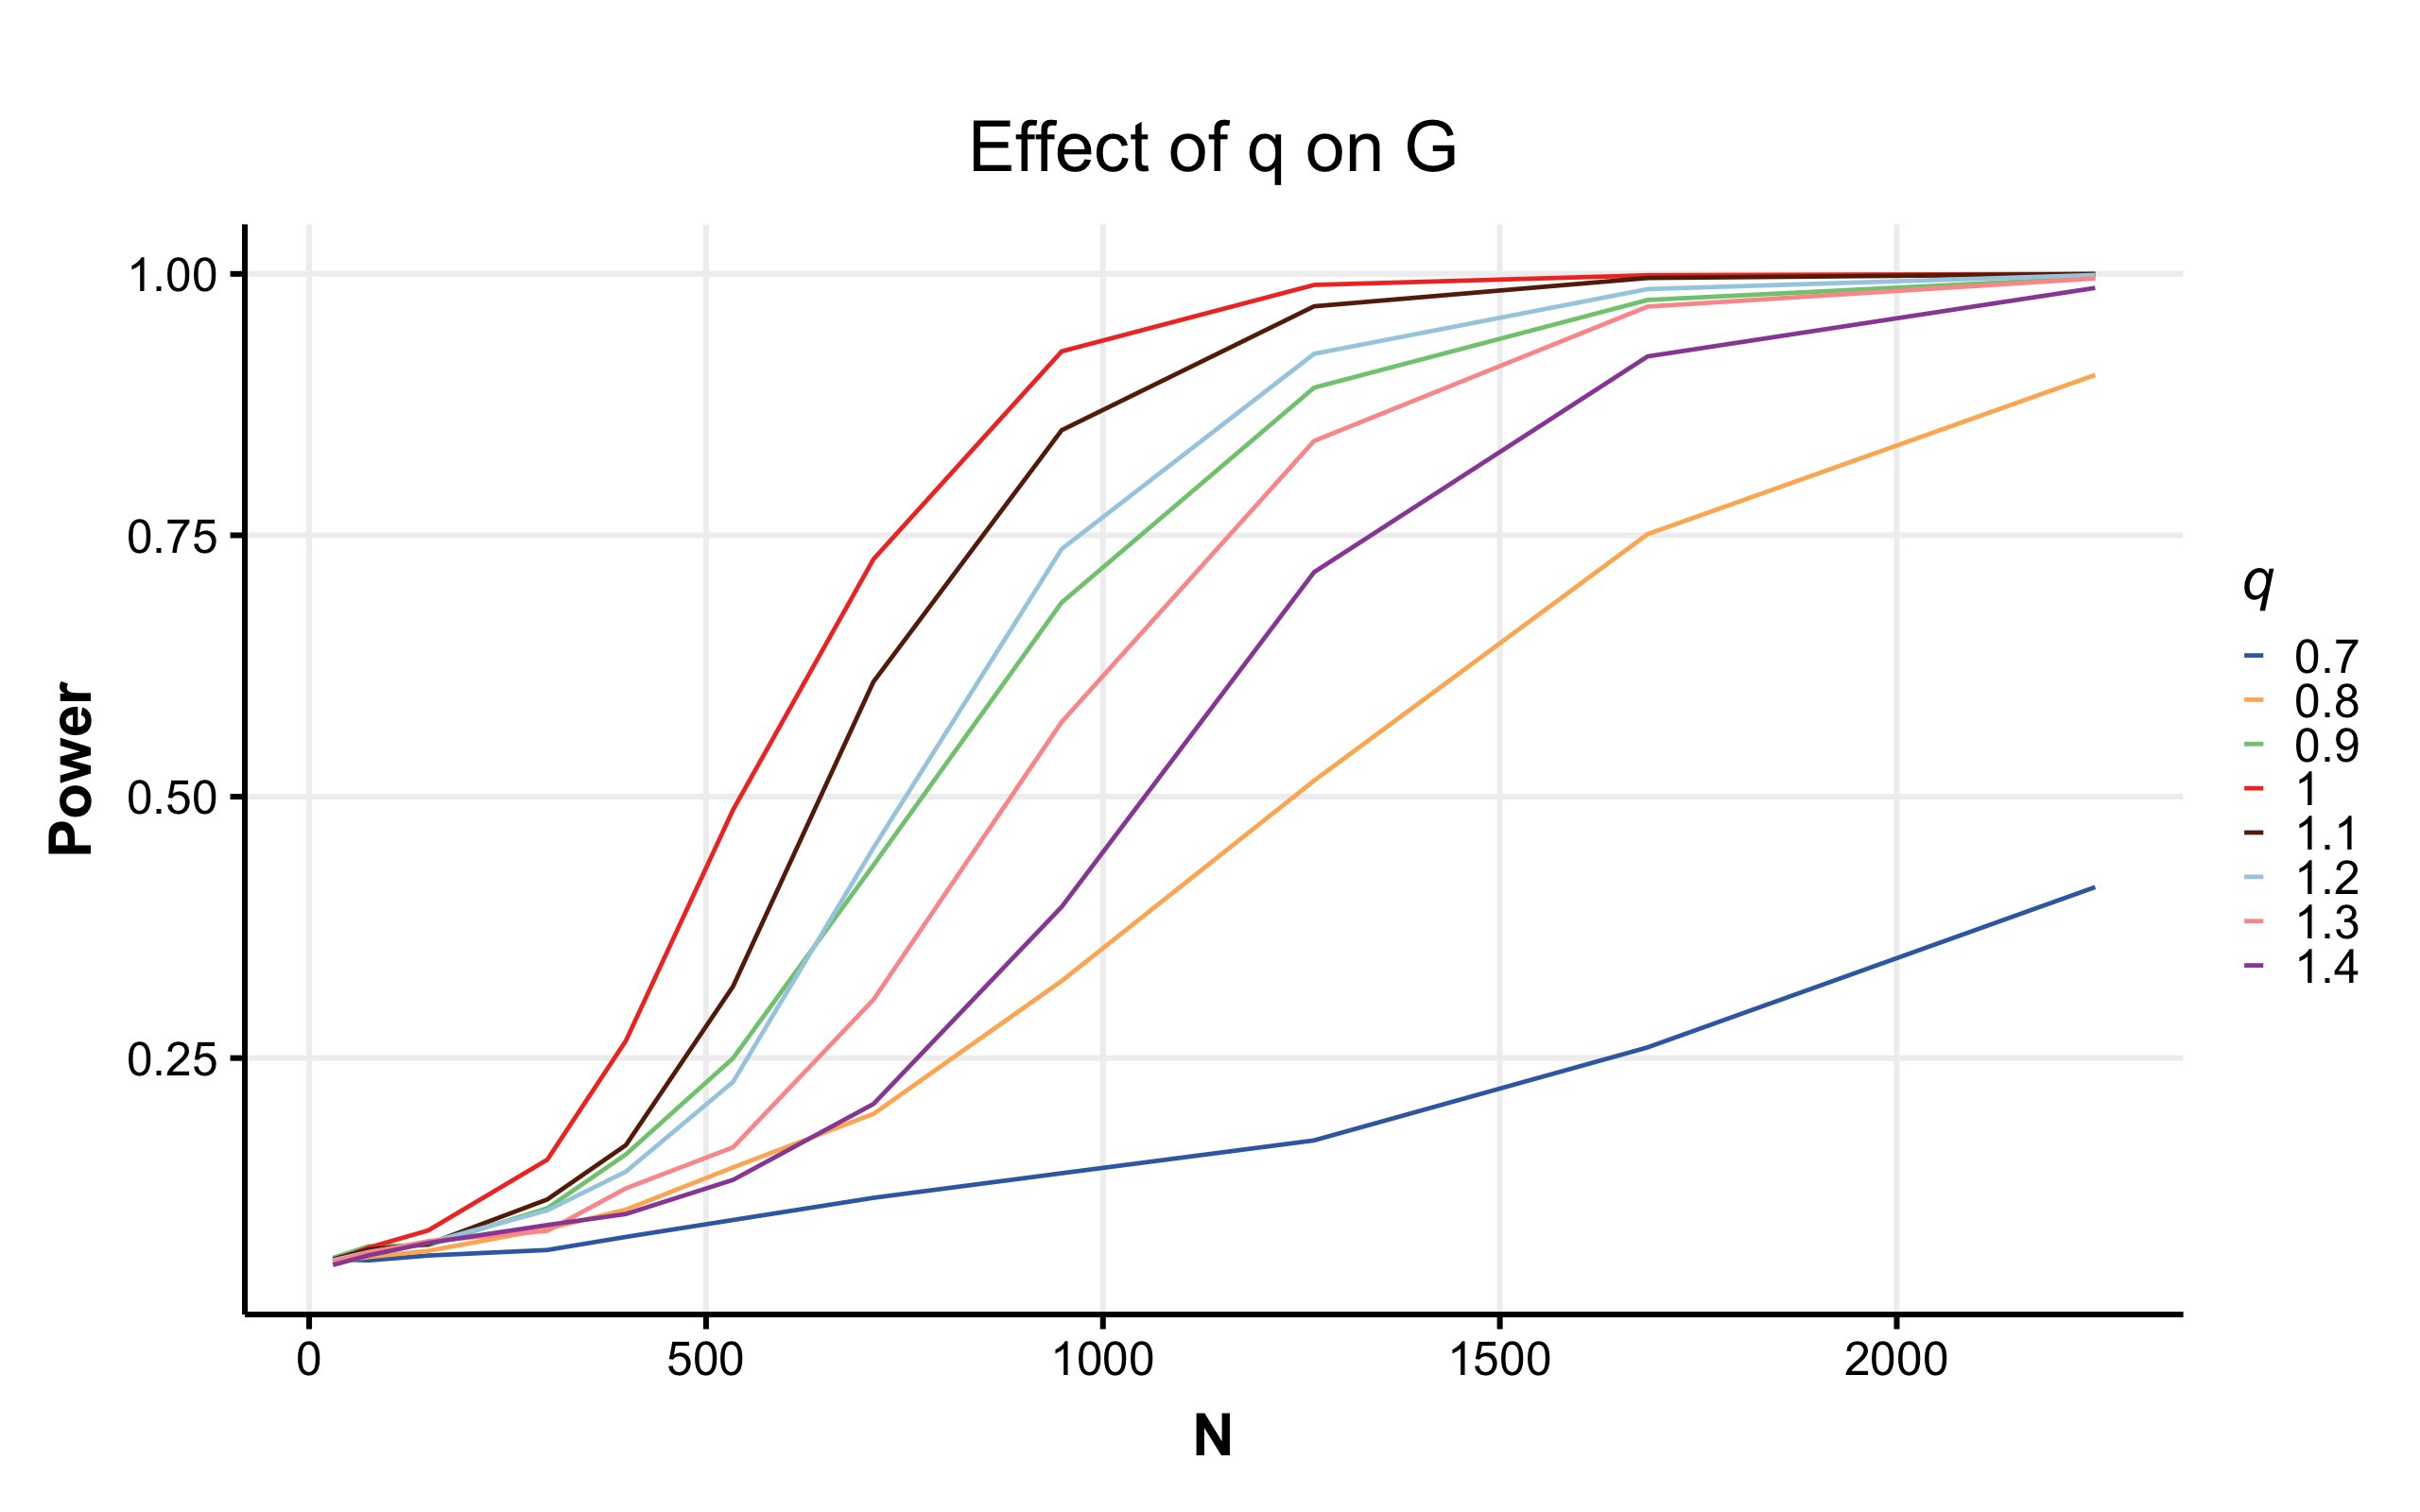
\includegraphics[width=\linewidth]  {g1-exponent.png}
\caption{The G-statistic's power is maximized when $q=1$. $\varepsilon = 1.$ }
\label{fig:Gpexponents}
\end{figure}

%\subsection{Optimal $\epsilon$ allocation for $G_1$-statistic}
We performed simulations to determine the ideal $\epsilon$ allocation between the $\var_1$ and \se calculations (Figure~\ref{Fig:g1-epsfrac}). Surprisingly, the results were different from the ideal allocation for the $F_1$-statistic. Across multiple group sizes and effect sizes, the effect of $\epsfrac$ was much less apparent. While using the default value of $\epsfrac = .5$ would be reasonable, our results suggest that minor improvement to power can be had by using $\epsfrac= 0.4$. %, i.e. $40\%$  of the epsilon budget going to the $\var_1$ calculation.

\begin{figure}
\centering
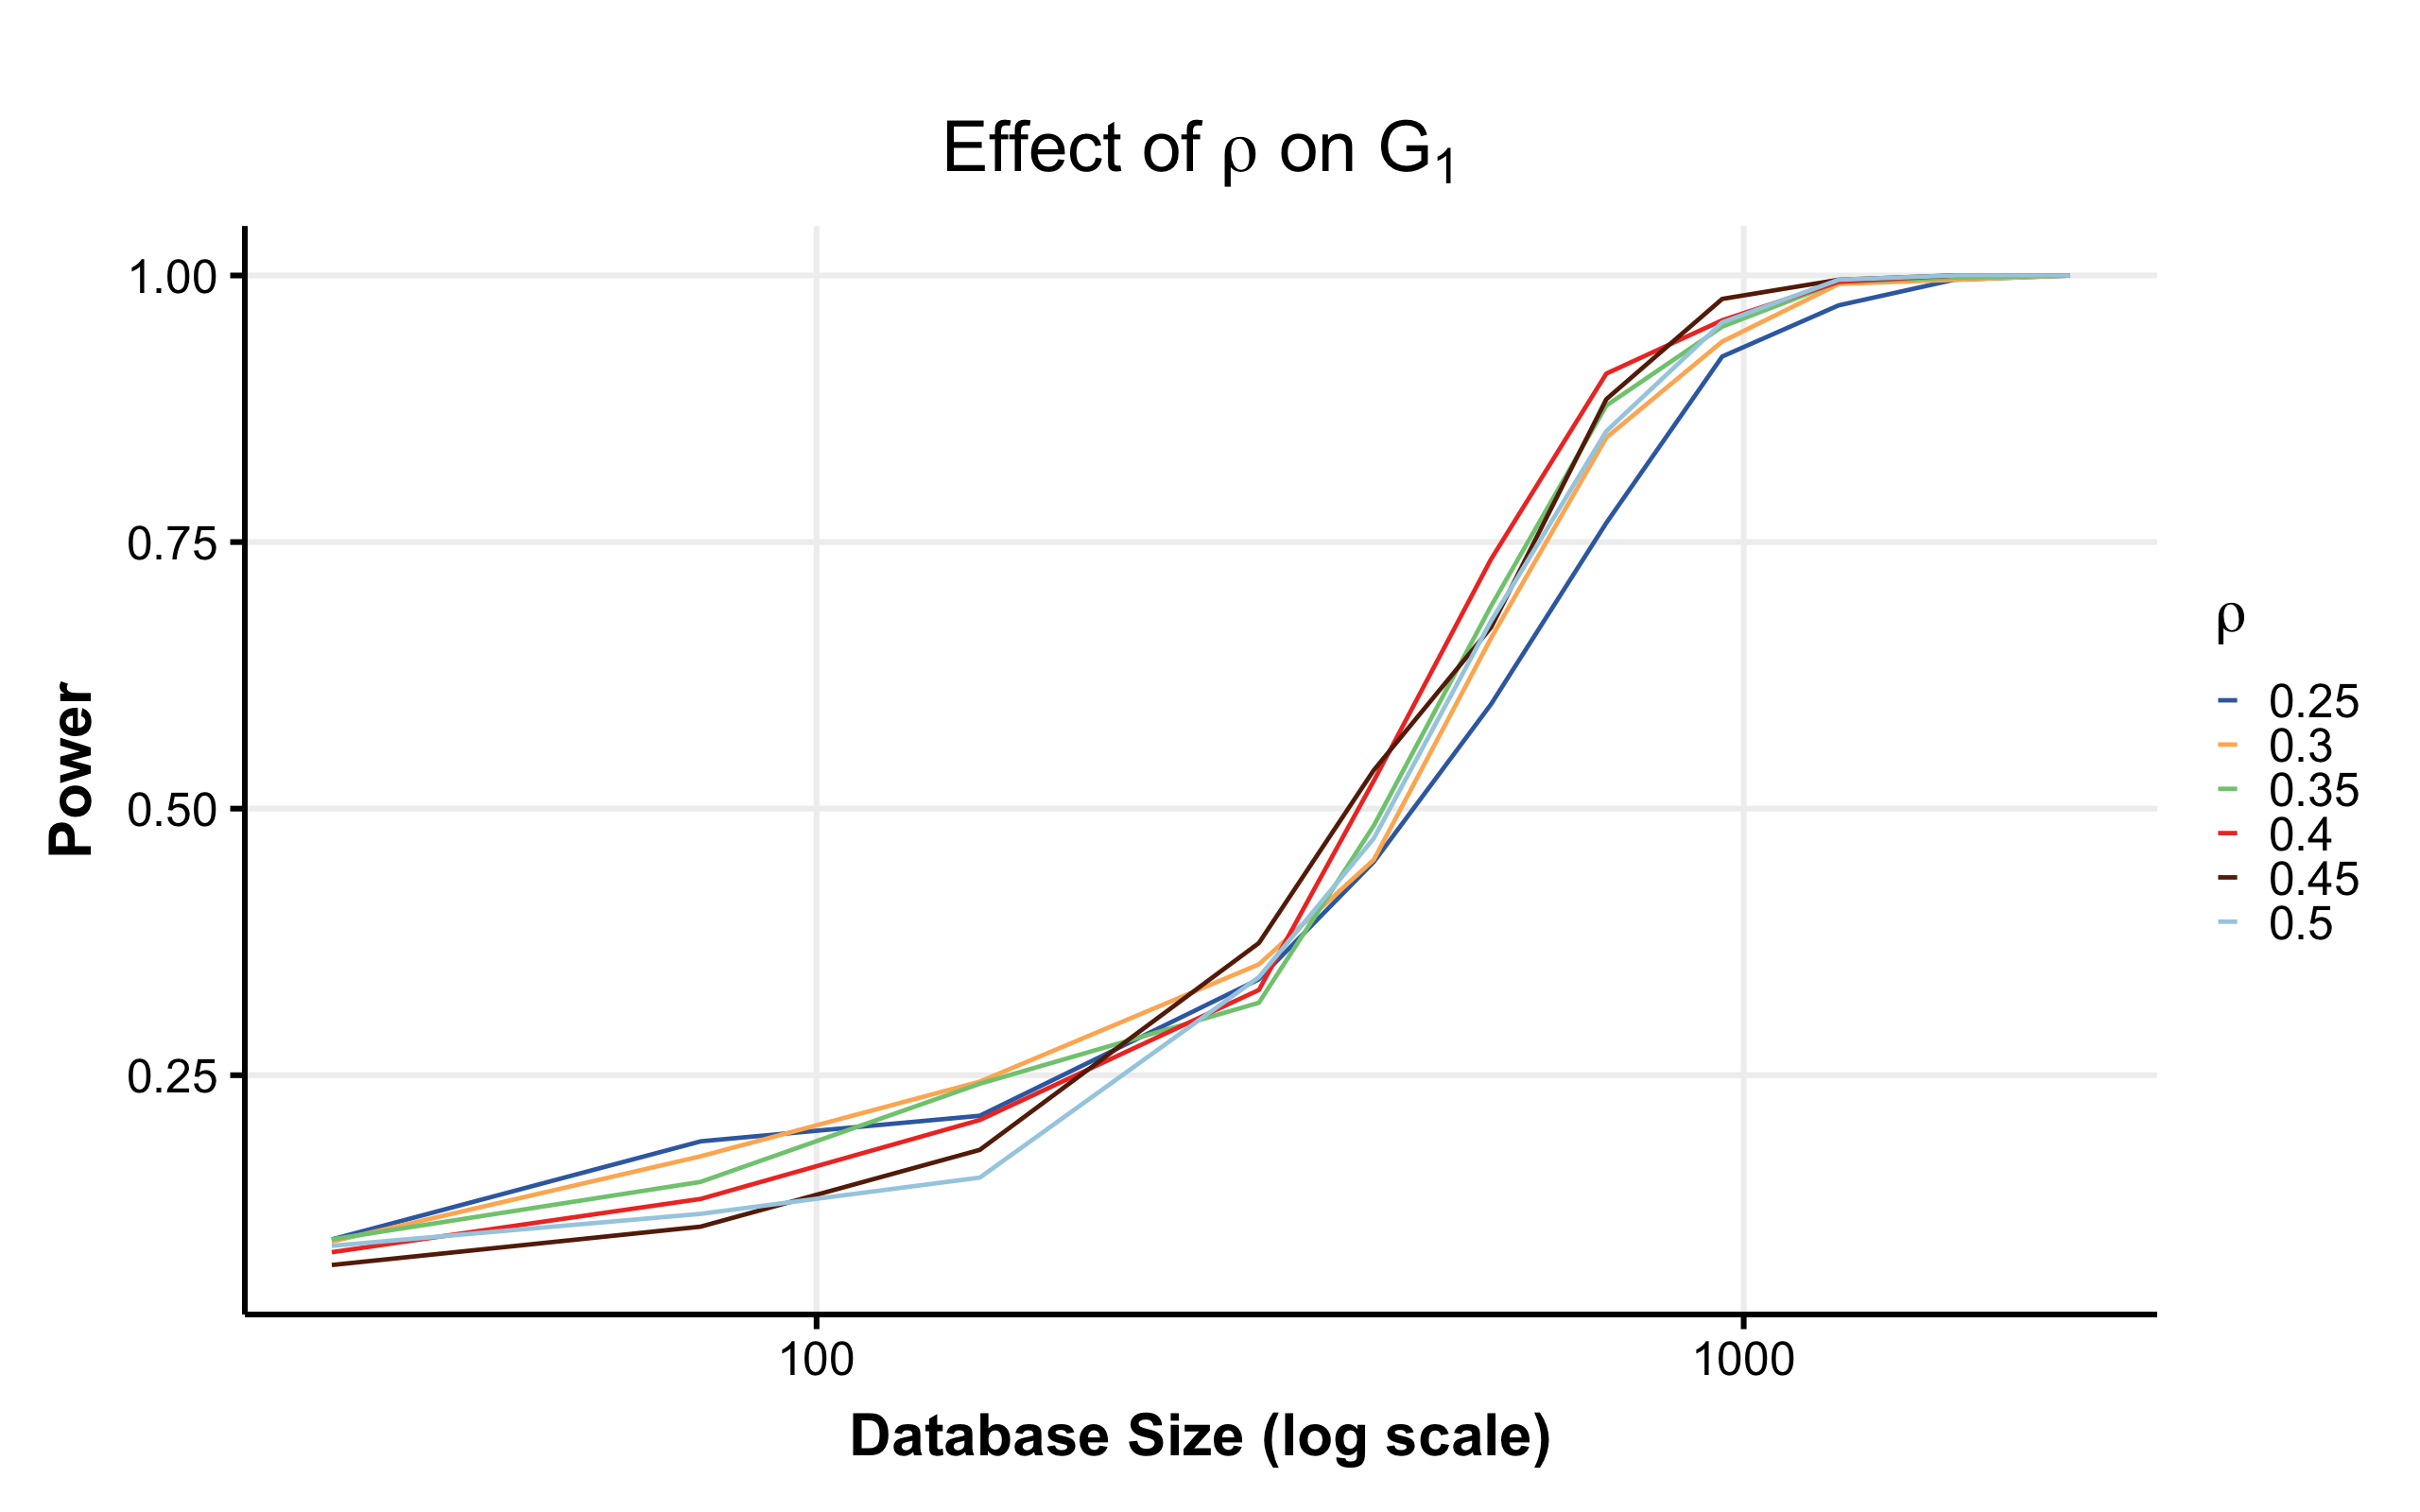
\includegraphics[width=.75\linewidth]{g1-epsfrac.png}
\caption{The power of $G_1$ at various choices of $\epsilon$ allocation.\label{Fig:g1-epsfrac}}
\end{figure}

%\subsection{Comparing $F_1$ and $G_1$}
While the $F_1$-statistic usually has more power than the $G_1$-statistic, there are some effect sizes for which the $G_1$-statistic has higher power. To investigate this fully, we considered the power of the two statistics across a large region of the practicable parameter space including $\sigma$ and effect size (Figure~\ref{Fig:f1-vs-g1}), as well as $k$ and $N$ (data not shown).

%In Figure~\ref{Fig:f1-vs-g1}, we highlight one of the rare regions of the parameter space where $G_1$ outperforms $F_1$. 

\begin{figure}
\centering
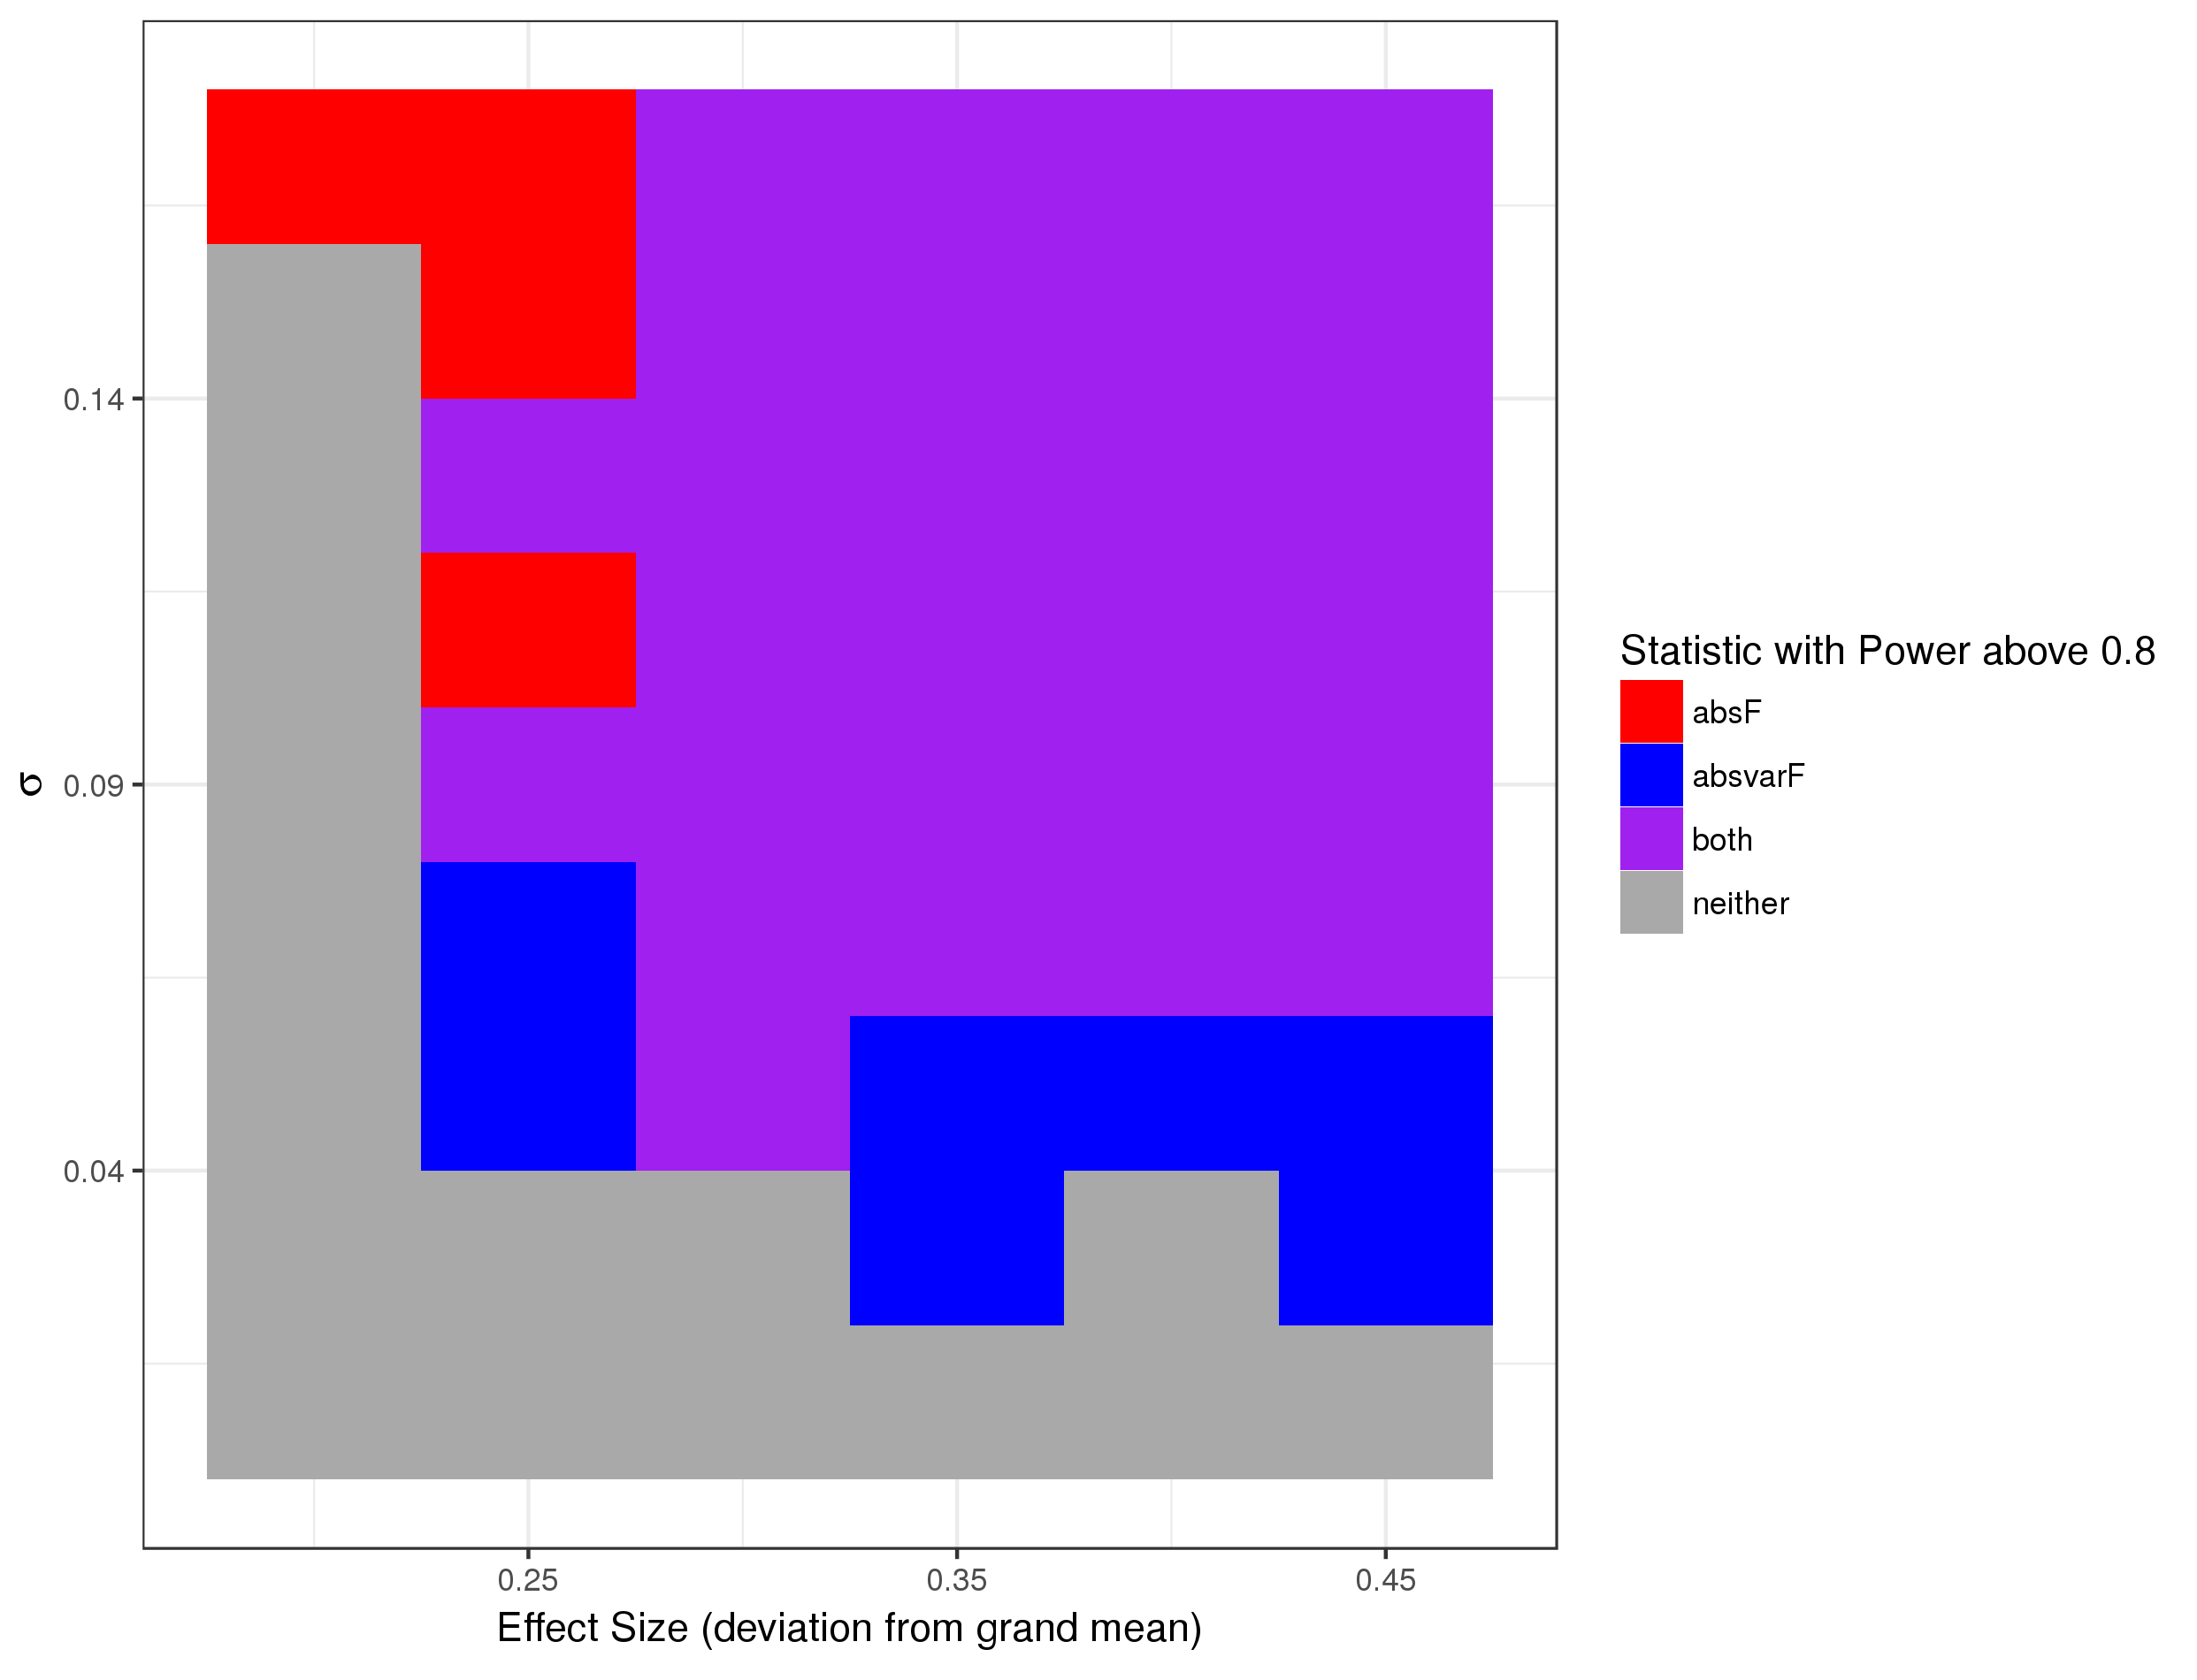
\includegraphics[width=\linewidth]{f1-vs-g1.png}
\caption{An image plot indicating which statistics achieve 80\% power at these particular paramter settings.\label{Fig:f1-vs-g1}}
\end{figure}